
\begin{minipage}{0.7\linewidth}
\section{Thyristoren}
Ein Thyristor besteh aus vier Halbleiterschichten d.h. aus drei pn-Übergängen\newline
Thyrisotren sind einschaltbare Bauelemente.\newline
Thyristoren sind  \" einschaltbare Dioden\". Thyristoren werden mit dem Zündimpuls der Zwischen Gate (G) und Kathode (K) kurzzeitig anliegt durchgeschalten.
\end{minipage}
\begin{minipage}{0.3\linewidth}
     \hspace{1cm}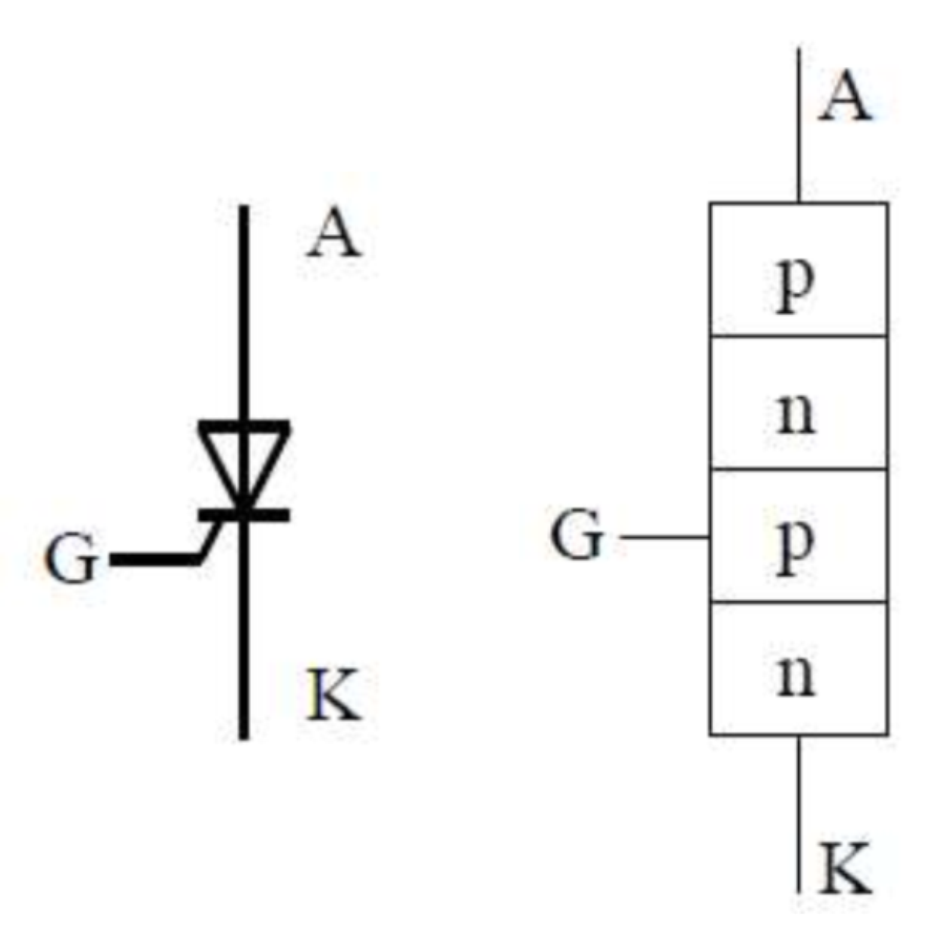
\includegraphics[width=0.5\linewidth]{images/thyraufbau}
\end{minipage}
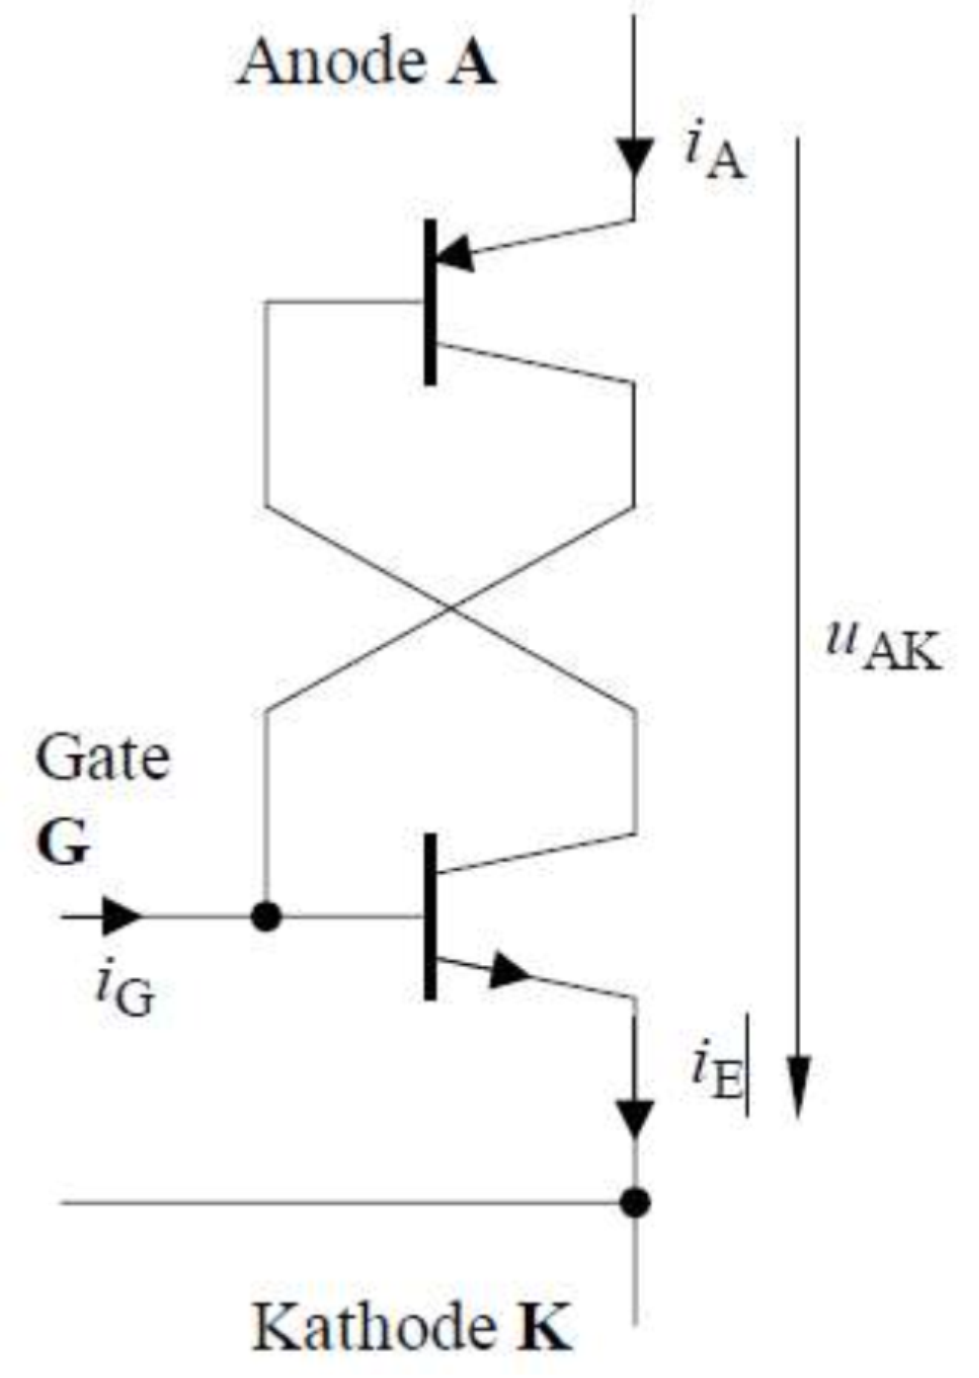
\includegraphics[width=0.15\linewidth]{images/thyrESB}
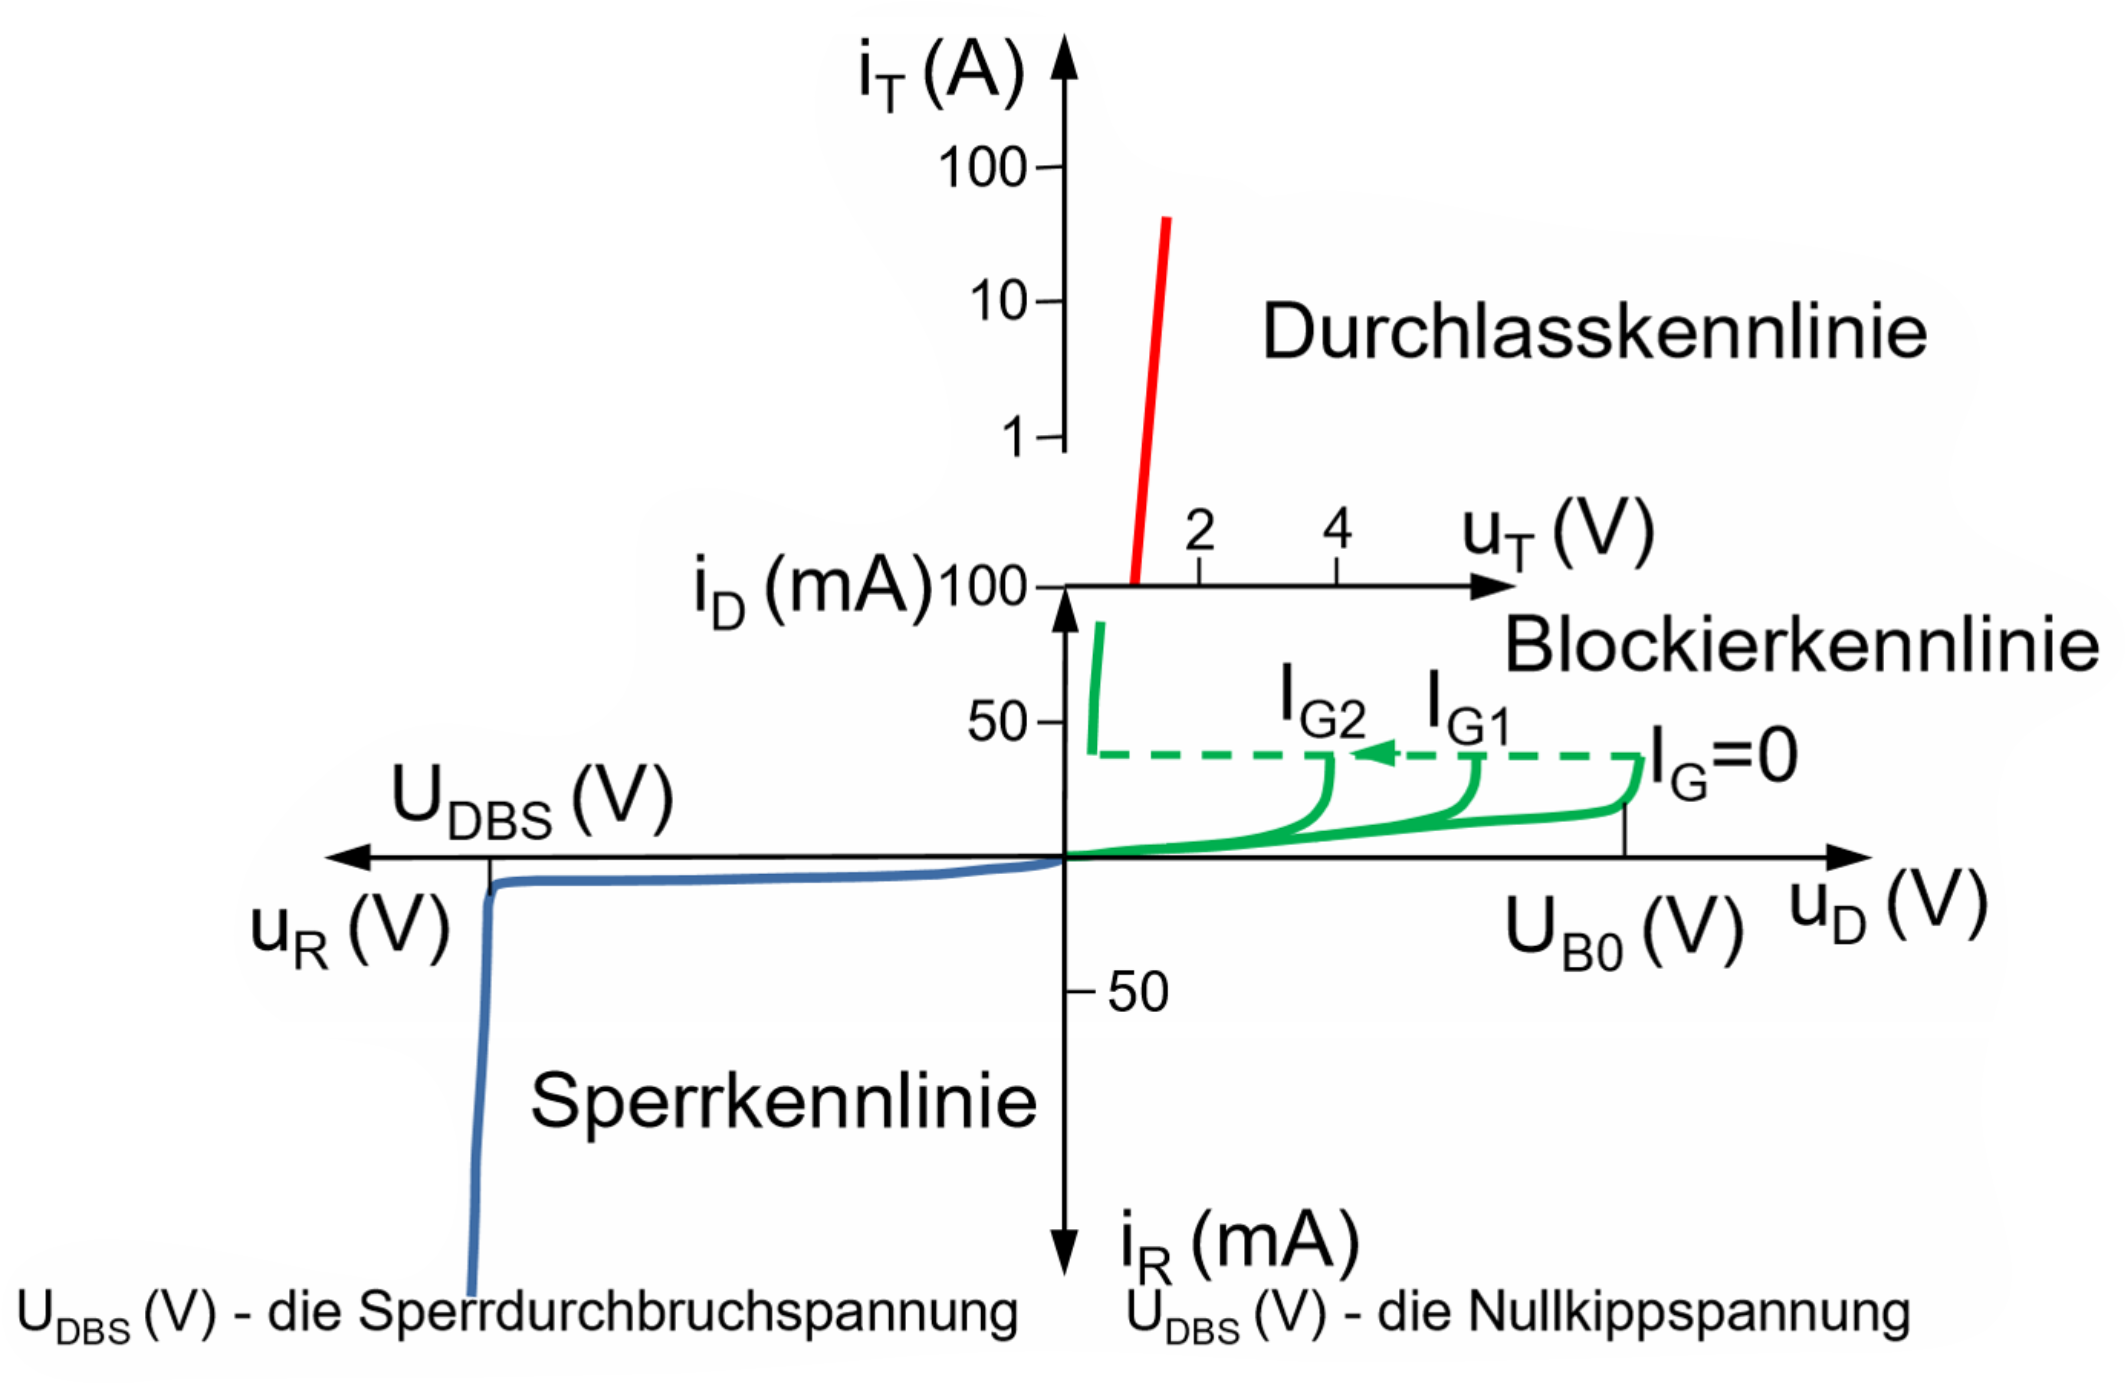
\includegraphics[width=0.4\linewidth]{images/thyrKennlinie}
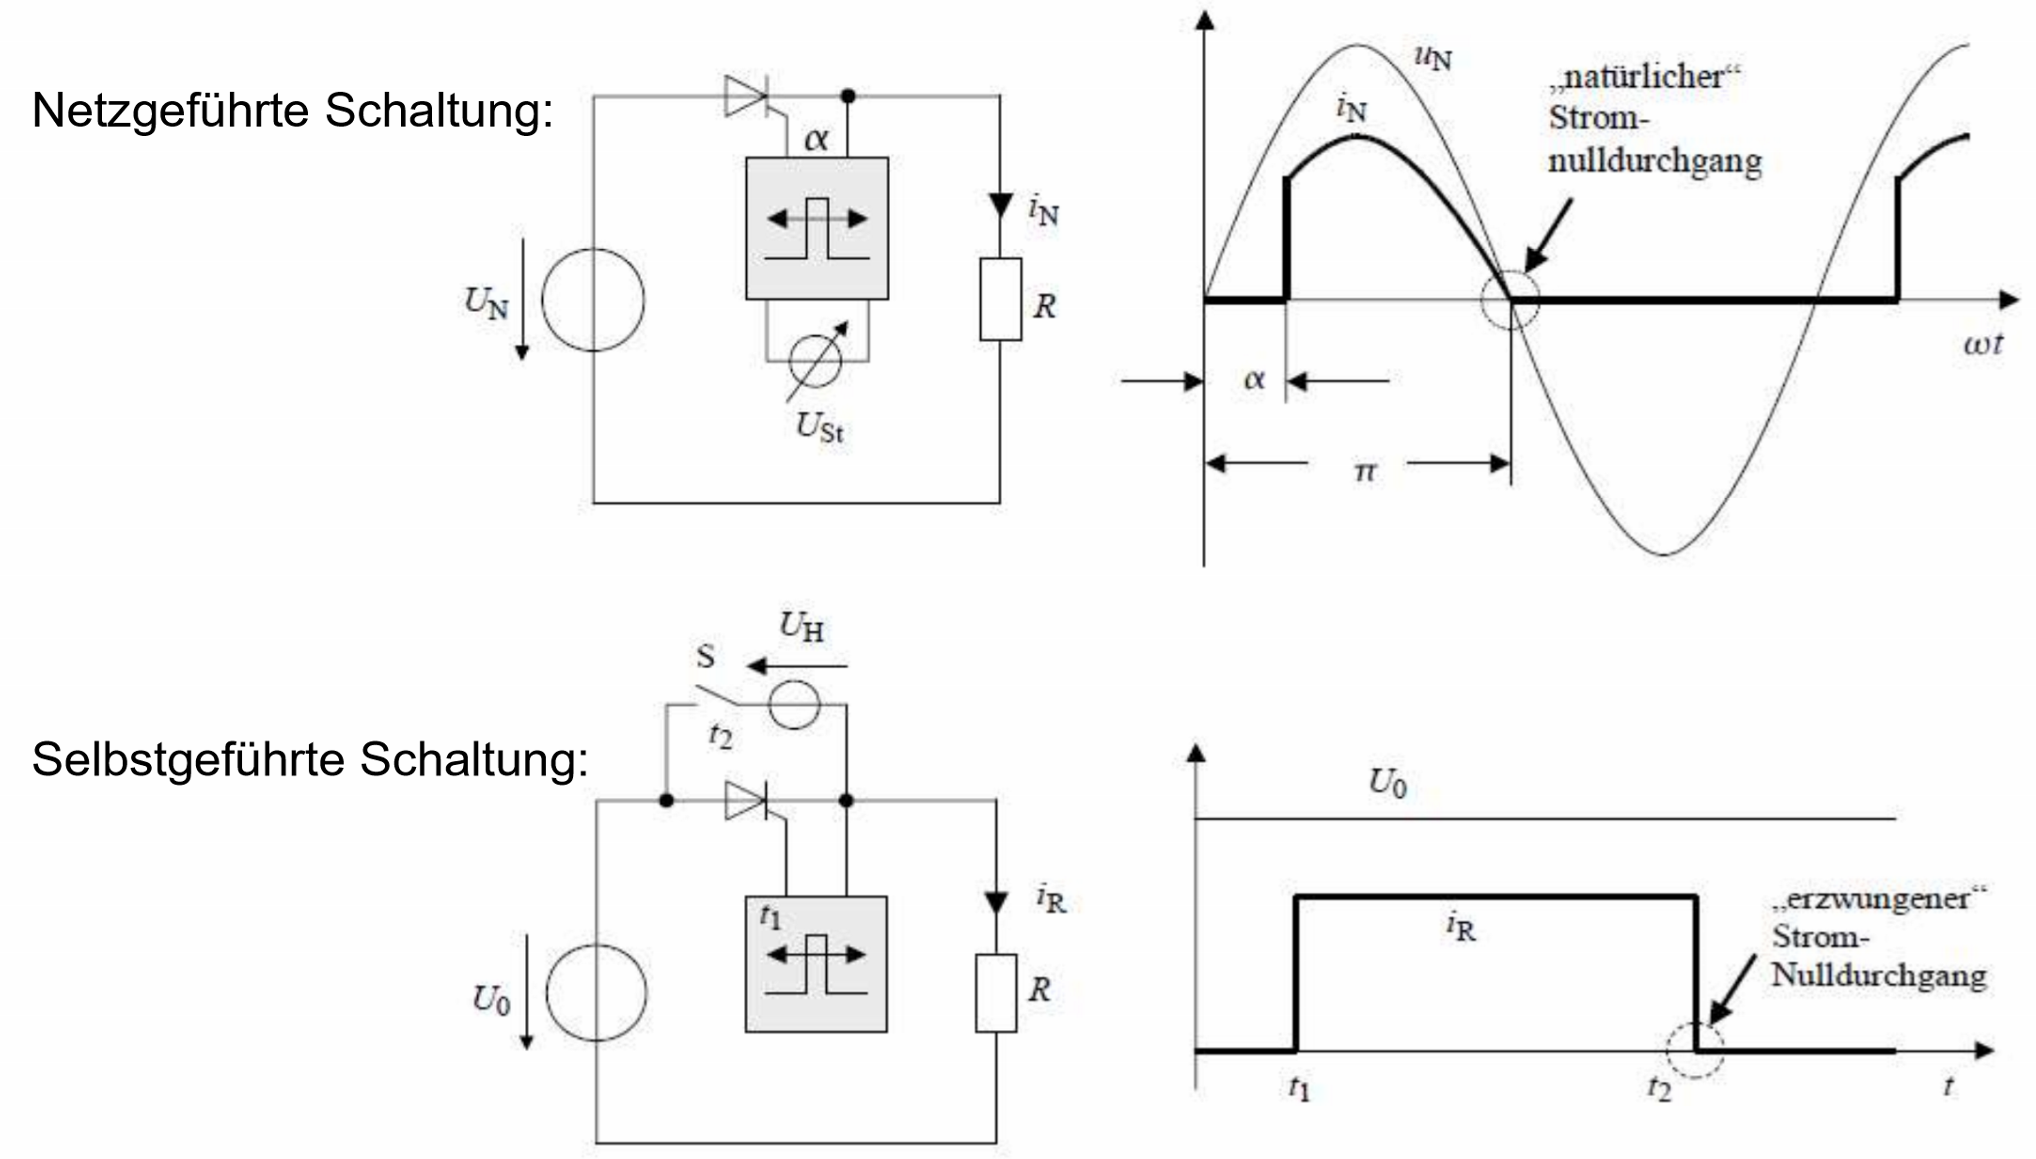
\includegraphics[width=0.45\linewidth]{images/thyrSchaltung}

\subsection{Thermische Eratzschaltung}
\begin{tabular}{p{7cm}l}
	\textbf{Thermische Kenngrösse}			& \textbf{Elektrische Kenngrösse}\\
	Wärmeleistung P [W]						& Strom I  [A]\\
	Temperaturunterschied $ \vartheta $[K] 	& Spannung [V]\\
	Wärmewiderstand $ R_{th} $ {K/W}		& Widerstand (V/A)\\
\end{tabular}

\begin{multicols}{2}
	\begin{minipage}{\linewidth}
		\subsubsection{Thyrisor ohne Kühlung}
		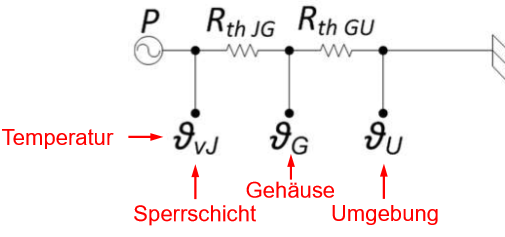
\includegraphics[width=0.6\linewidth]{images/thyrOK}
		\[ \vartheta_{vJ}-\vartheta_U=P \cdot (R_{th\; JG}+R_{th\; GU}) \]		
	\end{minipage}

	\begin{minipage}{\linewidth}
		\subsubsection{Thyrisor mit Kühlung}
		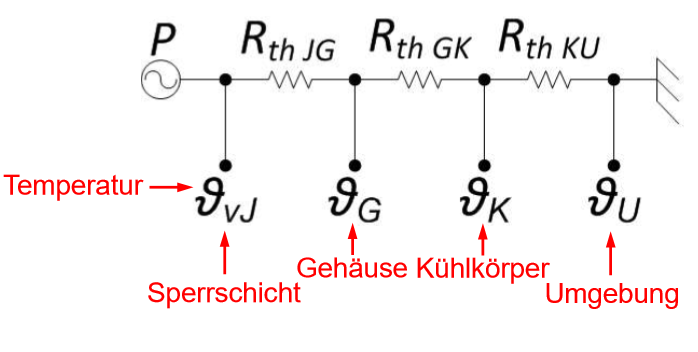
\includegraphics[width=0.6\linewidth]{images/thyrMK}
		\[ \vartheta_{vJ}-\vartheta_U=P \cdot (R_{th\; JG}+R_{th\; GK}+R_{th\; KU})\qquad R_{th \; KU}=\dfrac{\Delta \vartheta}{P} \]	
	\end{minipage}
\end{multicols}

\begin{minipage}{0.5\linewidth}
    \subsection{Abschaltbarer Thyristor}
    \begin{minipage}{0.7\linewidth}        
        \textbf{(GTO = Gate-Turn-Off)}\newline
        Der GTO Schaltet aus, wenn ein ausreichend hoher nagativer Gate-Strom auftritt.\newline
        Amplitude des Gate-Stromes muss 20\% bis 30\% des abzuschaltenden GTO-Stromes betragen.
    \end{minipage}
    \begin{minipage}{0.2\linewidth}
        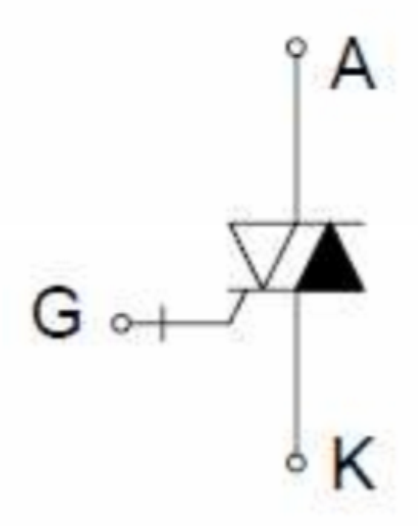
\includegraphics[width=\linewidth]{images/GTOSymbol}
    \end{minipage}    
\end{minipage}
\begin{minipage}{0.5\linewidth}
    \subsection{IGCT}
    \begin{minipage}{0.7\linewidth}
        \textbf{Integrated Gate-Commutated Thyristor}
        IGCT sind die Weiterentwicklung der GTO.\newline
        Sie werden hauptsächlich für Mittelspannungsumrichter iengesetzt.
    \end{minipage}
    \begin{minipage}{0.2\linewidth}
        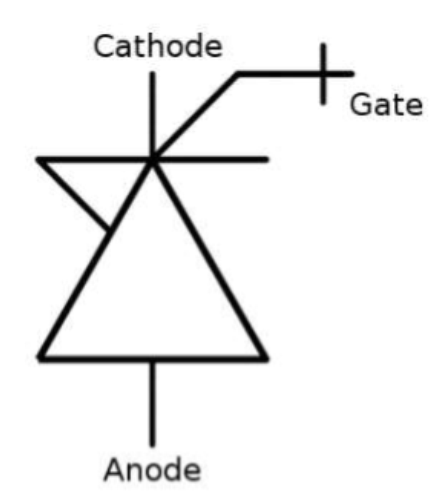
\includegraphics[width=\linewidth]{images/IGCTSymbol}
    \end{minipage} 
\end{minipage}
\clearpage
